\subsubsection{第一个例子}\label{twop}

我们首先考虑存在对称性破缺时两个初级场的情形。记这两个初级场的位置为 $z_1$ 与 $z_2$，并继续假定对称性破缺参数 $c$ 为正。只要 $z_1-z_2$ 不是实数，就存在一组对称选取的基本积分链 $\CC_a$，$a=1,2$：它们是从 $z_a$ 出发、平行于正实轴的射线。差 $\CC_1 - \CC_2= \CC_{12}$ 是从 $z_1 $ 到 $z_2$ 的线段。参见图~\ref{cyclesonetwo}。这三条链中的任意两条都可以成为针，取决于 $c$ 与 $z_1 - z_2$ 的相对大小。由于针始终只有两个，三条链 $\CC_1$、$\CC_2$ 与 $\CC_{12}$ 绝不可能同时都是针。

在这个简单的例子里，我们已经具备了一般辫群表示的基本要素。基本操作是交换两个 $z_a$，既可以顺时针也可以逆时针。我们从两个 $z_a$ 虚部互不相同的构型出发，这样各 $\CC_a$ 都良定义。不妨把 $z_a$ 的实部取为零。我们希望沿 $\CC_1$、$\CC_2$ 与 $\CC_{12}$ 定义 $\W$ 的分支，使得 $\CC_{12}=\CC_1-\CC_2$ 成立。在 $\CC_{12}$ 上任取 $\W$ 的一个分支，再在 $\CC_1$ 与 $\CC_2$ 上定义 $\W$，使它在 $\CC_1$ 与 $\CC_{12}$ 的唯一交点处、或在 $\CC_2$ 与 $\CC_{12}$ 的唯一交点处与前者一致。这就保证了 $\CC_{12}=\CC_1-\CC_2$。虽然 $\CC_1$ 与 $\CC_2$ 并不相交，但我们可以把它们稍作形变，使它们在右侧远处的某个参考点相遇，于是 $\W$ 的两个值在该参考点处一致。（这可由下述事实保证：可以把 $\W$ 定义为在以 $\CC_1$、$\CC_2$ 与 $\CC_{12}$ 为界的半无限矩形内单值。）

% [Tutor Note: 含糊点拨] 作者说“这可由……单值保证”而略去论证，实质是：$\CC_1$、$\CC_2$ 与“无穷远处的连接段”围成的半无限矩形内 $\W$ 没有临界点，故沿该矩形边界一周 $\W$ 的单值性成立；令无穷远处的连接段收缩，即得两个参考点处 $\W$ 的取值相等。若该矩形内存在临界点，这一论证失效，正是后文 $|Z|<<1$ 时出现额外临界点的原因。

设 $\mathrm{Im}\,( z_1-z_2)>0$。那么我们可以用两种方式穿到 $\mathrm{Im}\,( z_1-z_2)<0$，即让 $z_1$ 从 $z_2$ 的左侧或右侧绕过。这两个操作互为逆操作，因此详细考察其中一个就够了。若 $z_1$ 从 $z_2$ 的右侧绕过，则 $\CC_1$ 作为一条平行于正实轴的射线连续演化。另一方面，$\CC_2$ 则不然。我们可以改用 $\CC_{12}$，它被连续地定义为从 $z_1$ 到 $z_2$ 的线段。在 $\CC_1$ 与 $\CC_{12}$ 这组基下，这一编织操作是对角的：我们只需追踪 $\W$ 的分支与链的取向。我们想把最终结果用 $\CC_1$ 与 $\CC_2$ 的基来表达。

在半编织中，$\CC_1$ 乘以因子 $q^{-\frac{1}{4}}$：$z_1$ 被顺时针地绕 $z_2$ 输运，而参考点没有显著移动。半编织之后，我们把 $\CC_1$ 重新命名为 $\CC_2$：
\begin{equation}\label{elfin}
\CC_1 \to q^{-\frac{1}{4}} \CC_2.
\end{equation}

% [Tutor Note: 易错点] 这里指数是 $-1/4$，来源是超势中的 $-\frac12\log(z_1-z_2)$ 项：$z_1$ 顺时针绕过 $z_2$ 半圈时，$z_1-z_2$ 顺时针转过 $\pi$，故 $\log(z_1-z_2)$ 改变 $-i\pi$，于是 $-\frac12\log(z_1-z_2)$ 改变 $+\frac{i\pi}{2}$，$\exp(\W/b^2)$ 乘以 $e^{\pi i/(2b^2)}=q^{-1/4}$（用 $q=e^{-2\pi i/b^2}$ 检验）。若把编织方向取反（逆时针），该因子及其后所有公式的指数符号都要整体翻转；这正是下文 (\ref{zolt}) 与 (\ref{cmono}) 相比指数符号相反的原因（作者已说明两次推导的编织方向相反）。

\begin{figure}
 \begin{center}
     % >>> 原文图 10（原稿第 65 页）
  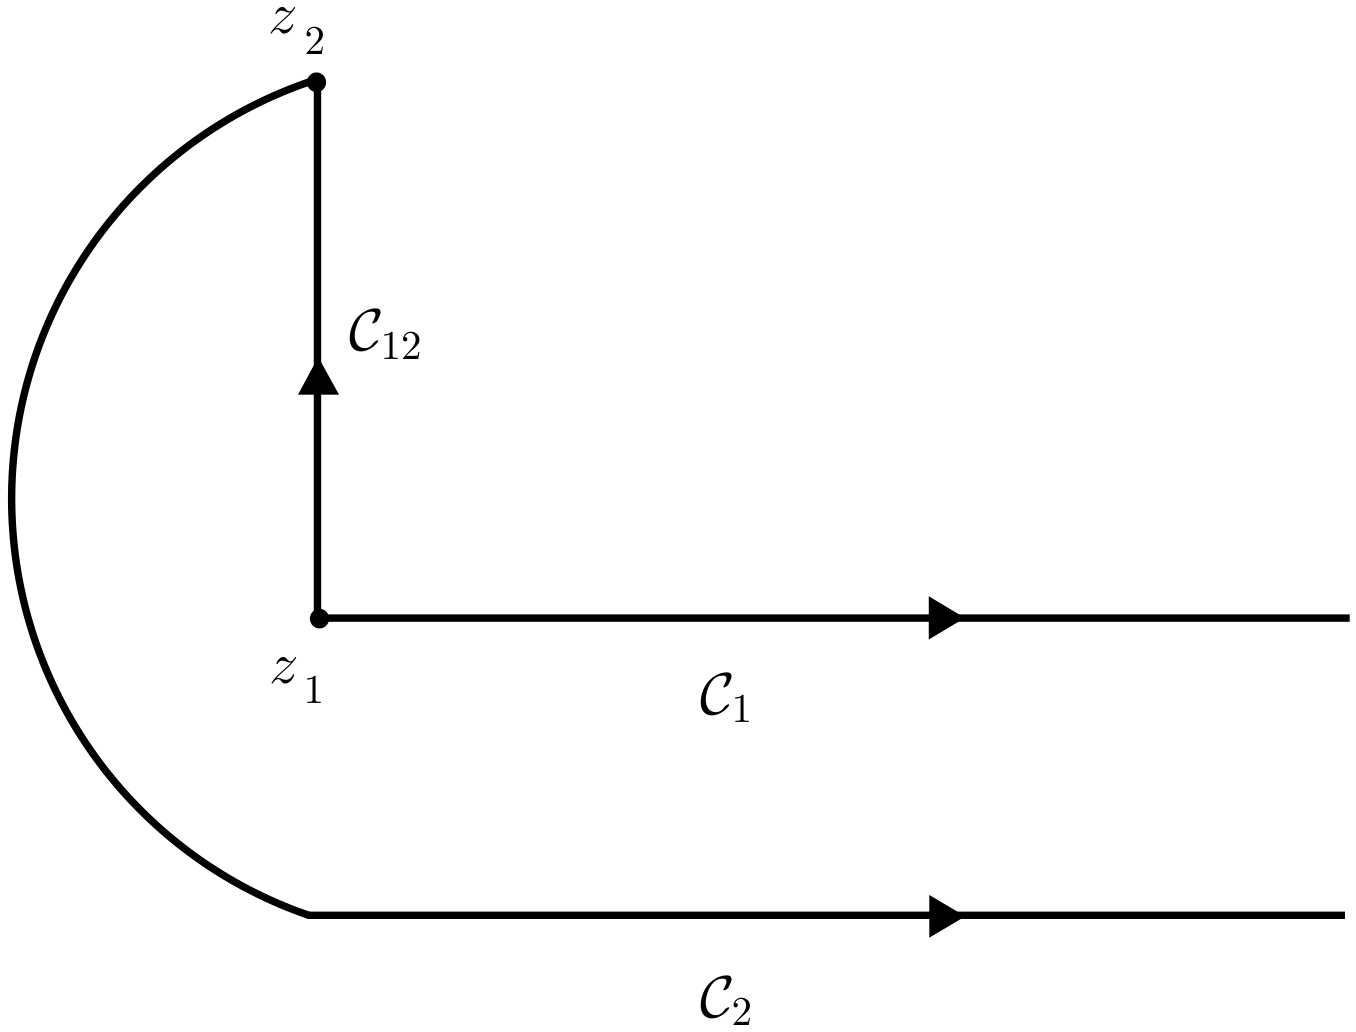
\includegraphics[width=3.5in]{figs/Fig10.png}
 \end{center}
\caption{\small 一次编织操作之后的链 $\CC_1$、$\CC_2$ 与 $\CC_{12}$。（原稿第 65 页）}
 \label{cyclesonetwob}
\end{figure}

\begin{figure}
 \begin{center}
     % >>> 原文图 11（原稿第 66 页）
  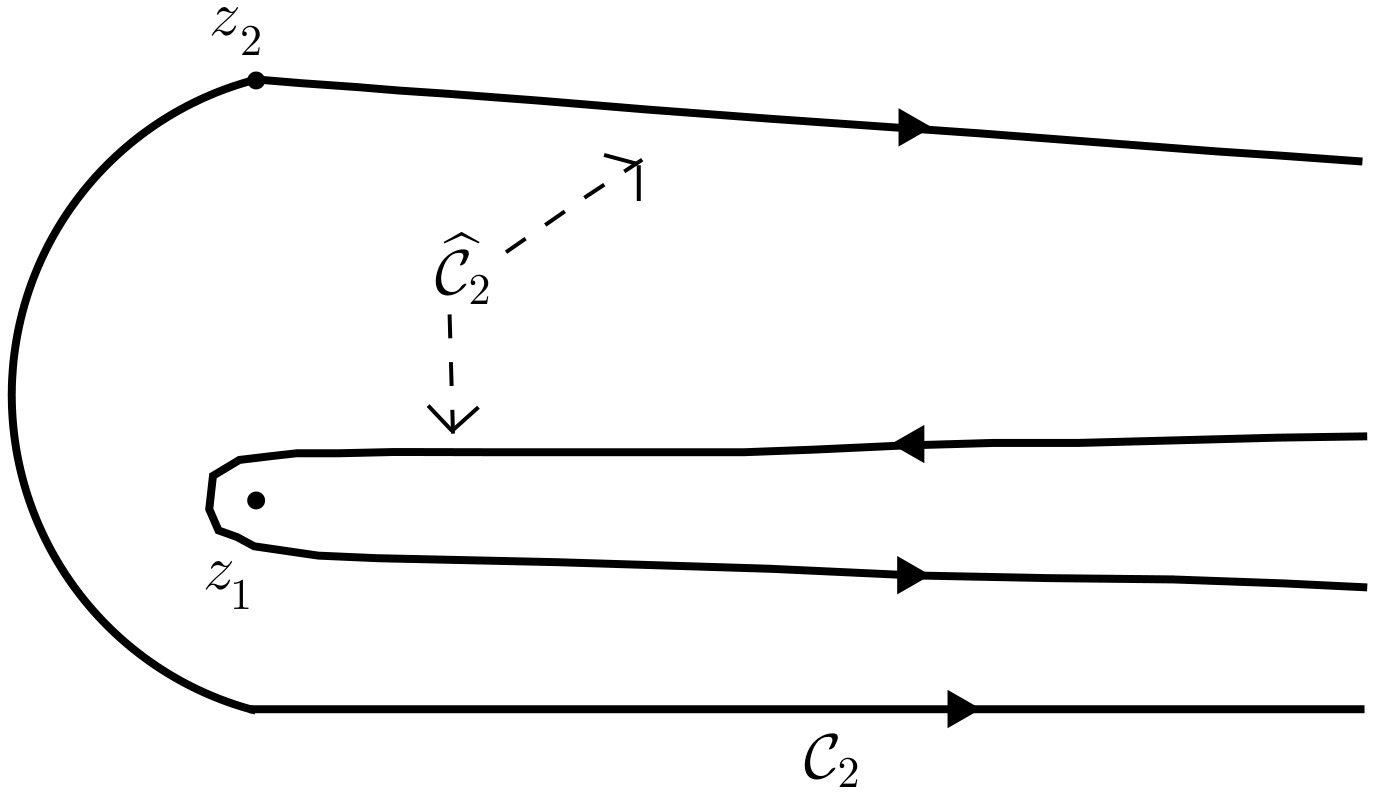
\includegraphics[width=3.5in]{figs/Fig11.png}
 \end{center}
\caption{\small 编织操作之后的链 $\CC_2$ 是照图~\ref{cyclesonetwob} 复制而来的：它从 $z_2$ 出发，从 $z_1$ 下方弯向左侧，然后通向 $\mathrm{Re}\,z=\infty$。它在同调意义下等价于图中标记为 $\widehat\CC_2$ 的锯齿形链：后者从 $z_2$ 出发，先径直通向 $\mathrm{Re}\,z=\infty$，再折返绕过 $z_1$，最后又回到 $\mathrm{Re}\,z=\infty$。于是 $\widehat\CC_2$ 是三段之和，每一段都通向或来自 $\mathrm{Re}\,z=\infty$；每一段都等价于 $q$ 的某个幂次乘以基本链 $\CC_1$ 或 $\CC_2$（即从 $z_1$ 或 $z_2$ 出发、平行于正 $z$ 轴的射线）。（原稿第 66 页）}
 \label{cyclesonetwoc}
\end{figure}

另一方面，$\CC_2$ 变成图~\ref{cyclesonetwob} 中的链。它可以形变为三段之和，这三段锯齿般地往返于 $\mathrm{Re}\,z=\infty$，如图~\ref{cyclesonetwoc} 所示。三段中的每一段都等价于 $q$ 的某个幂次乘以原链 $\CC_1$ 与 $\CC_2$ 之一。正如 (\ref{elfin}) 那样，其中一段（在再一次交换 $\CC_1$ 与 $\CC_2$ 的标号之后）是 $q^{-\frac{1}{4}} \CC_2$。另外两段则是 $-q^{-\frac{1}{4}} \CC_2$ 与 $q^{-\frac{1}{4}} \CC_1$ 在某个覆盖变换下的像。因此编织变换为
\begin{equation}
\CC_2 \to q^{-\frac{1}{4}} \CC_2-  q^{\frac{3}{4}} \CC_2 + q^{\frac{3}{4}} \CC_1.
\end{equation}

注意，在这些变换规则下，
\begin{equation}\label{zolt}
\CC_{12} \to -  q^{\frac{3}{4}} \CC_{12}.
\end{equation}
这与我们在式 (\ref{cmono}) 中得到的结果相同（指数的符号相反，因为在推导 (\ref{zolt}) 时我们是让 $z_1$ 顺时针地绕 $z_2$ 编织的）；对称性破缺并不影响下述事实：$\CC_{12}$ 代表两个退化场融合为恒等场的共形块。编织矩阵的本征值为 $-  q^{\frac{3}{4}}$ 与 $q^{-\frac{1}{4}}$，它们对应于两个可能的融合道。线性组合 $\CC_1 + q^{-1} \CC_2$ 的变换为
\begin{equation}
\CC_1 + q^{-1} \CC_2 \to q^{-\frac{1}{4}} (\CC_1 + q^{-1} \CC_2).
\end{equation}
因此它代表动量为 $-b$ 的道中的融合。

% [Tutor Note: 易错点] 两个本征值 $-q^{3/4}$ 与 $q^{-1/4}$ 分别对应恒等道（$\CC_{12}$）与动量为 $-b$ 的道（$\CC_1+q^{-1}\CC_2$）。校验可用两个不变量：在基 $(\CC_1,\CC_2)$ 下，由变换规则读出的迹为 $q^{-1/4}-q^{3/4}$、行列式为 $-q^{1/2}$，恰好等于 $(-q^{3/4})+q^{-1/4}$ 与 $(-q^{3/4})(q^{-1/4})$。注意恒等道的本征值带负号且指数为 $+3/4$；与 (\ref{cmono}) 比较时须把编织方向反过来，符号与指数才都会对上。

现在，$\CC_1$ 与 $\CC_2$ 的其他归一化选择在各种情形下可能更自然地出现。若改变 $\CC_1$ 与 $\CC_2$ 之间的相对归一化，例如令 $\tilde \CC_1 = q^{-s/2} \CC_1$ 与 $\tilde \CC_2 = q^{s/2} \CC_2$，则可以得到编织公式
\begin{equation}\label{furthox}
B_{12} :~~ \tilde \CC_1 \to q^{-s-\frac{1}{4}} \tilde \CC_2
\qquad   \tilde \CC_2 \to \left( q^{-\frac{1}{4}} -  q^{\frac{3}{4}} \right)
\tilde \CC_2 + q^{s+\frac{3}{4}} \tilde \CC_1.
\end{equation}
我们马上就会发现 $s=-\frac{1}{2}$ 这一选择很有用，因此此后每当写 $\tilde \CC_a$ 时，我们都采用该 $s$ 值。

\begin{figure}
 \begin{center}
     % >>> 原文图 12（原稿第 67 页）
  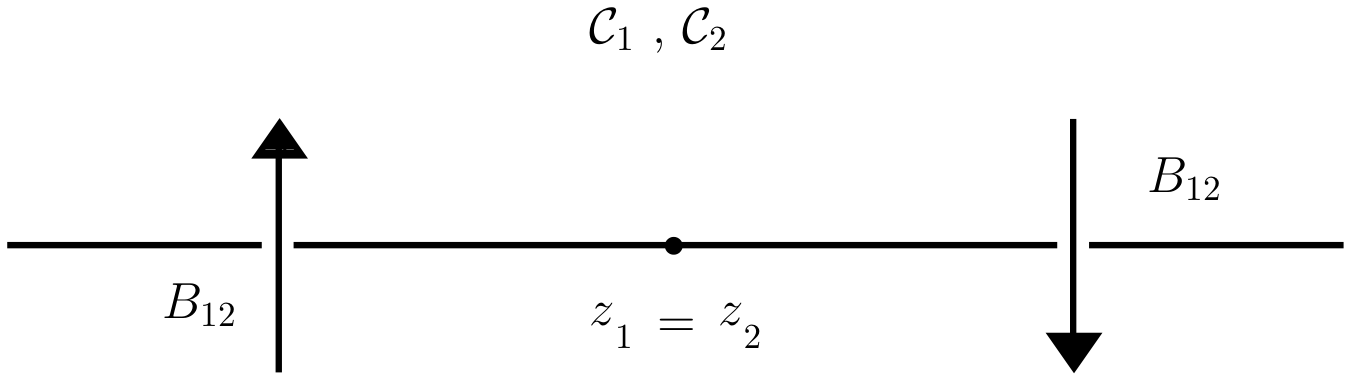
\includegraphics[width=3.5in]{figs/Fig12.png}
 \end{center}
\caption{\small 链 $(\CC_1,\CC_2)$（定义为从 $z=z_1$ 或 $z_2$ 出发、沿 $\mathrm{Re}\,cz$ 方向的射线）为同调提供了一个局部基，但穿越使 $Z=c(z_1 - z_2)$ 为实数的直线时，链的定义会跳跃一个编织矩阵 $B_{12}$。（原稿第 67 页）}
 \label{braida}
\end{figure}

各 $\CC_a$ 作为 $c(z_1 - z_2)$ 的函数的行为如图~\ref{braida} 所示。当 $c(z_1-z_2)$ 为实数时，各 $\CC_a$ 不再是良定义的。在这个非常简单的例子里，沿 $\CC_a$ 的积分可以显式地用熟知的函数表示：
\begin{align}
\I_a &= \oint_{\CC_a} (w-z_1)^{\frac{1}{b^2}}(w-z_2)^{\frac{1}{b^2}}
(z_1-z_2)^{-\frac{1}{2b^2}} e^{\frac{c z_1}{2} + \frac{c z_2}{2} - c w} \d w \cr &= c^{-1 - \frac{3}{2 b^2}} \oint_{\CC_a} (W-Z)^{\frac{1}{b^2}}W^{\frac{1}{b^2}}Z^{-\frac{1}{2b^2}} e^{\frac{Z}{2} - W} \d W 
\end{align}
这里我们定义了 $W = c(w-z_2)$ 与 $Z = c(z_1 - z_2)$。这个积分可以显式地用 Bessel 函数写出。沿 $\CC_1$ 与 $\CC_2$ 的积分给出大 $Z$ 下具有特定渐近行为的一组 Bessel 函数基，而编织矩阵 $B$ 捕捉的正是 Bessel 函数的 Stokes 现象：
\begin{align}
\I_1 &= \frac{1}{\sqrt{\pi } c^{1 + \frac{3}{2 b^2}}} Z^{\frac{1}{2 b^2}+\frac{1}{2}} \Gamma \left(1+\frac{1}{b^2}\right)
   K_{\frac{1}{2}+\frac{1}{b^2}}\left(\frac{Z}{2}\right) \cr 
   \I_2 &= \frac{q^{1/4}}{\sqrt{\pi } c^{1 + \frac{3}{2 b^2}}} Z^{\frac{1}{2 b^2}+\frac{1}{2}} \Gamma \left(1+\frac{1}{b^2}\right)
   K_{\frac{1}{2}+\frac{1}{b^2}}\left(-\frac{Z}{2}\right) 
\end{align}

% [Tutor Note: 省略证明] 从第一式到第二式（$W,Z$ 的替换）并不只是变量替换：$e^{\frac{c z_1}{2}+\frac{c z_2}{2}-cw}$ 是超势的指数化形式，代入 $W=c(w-z_2)$ 时会产生 $c$ 的幂次因子 $c^{-1-\frac{3}{2b^2}}$，其中 $-1$ 来自 $\d w=c^{-1}\d W$，$-\frac{3}{2b^2}$ 来自三个 $W,Z$ 因子的组合幂次。作者略去了这一步的幂次记账；若漏掉 $c$ 的幂，Bessel 表达式前的系数就会与原文差一个 $c$ 因子。

在大 $Z$ 极限下，沿 $\CC_a$ 的积分由 $w$ 靠近 $z_a$ 的区域所主导。取对数的一个分支使超势中对数之和在 $w$ 接近 $z_1$（或 $z_2$）时趋于 $\frac{1}{4} \log(z_1 - z_2)^2$，这样做是有用的。这与 $s=-\frac{1}{2}$ 时 $\CC_a$ 与 $\tilde \CC_a$ 之间的归一化改变相同。在强对称性破缺时，$\tilde \CC_a$ 这组基会很有用。在此基下
\begin{equation}\label{nurth}
B_{12} := \tilde \CC_1 \to q^{\frac{1}{4}} \tilde \CC_2  \qquad   \tilde \CC_2 \to \left( q^{-\frac{1}{4}} -  q^{\frac{3}{4}} \right) \tilde \CC_2 + q^{\frac{1}{4}} \tilde \CC_1.
\end{equation}

到目前为止，我们所用的链 $\CC_1$、$\CC_2$ 与 $\CC_{12}$ 都是凭观察就能看出的。让我们把这些链与针作比较。含两个 $z$ 与一个 $w$ 的 Bethe 方程为
\begin{equation}
\frac{1}{w - z_1} + \frac{1}{w - z_2} =c
\end{equation}
它有两个解。

有两个值得关注的区域。若 $|Z|>>1$，则临界点近似为 $w = z_a + 1/c$，$a=1,2$。对这两个临界点中的每一个，假定 $c>0$ 且 $\mathrm{Re}\,Z=0$，则 $w-z_1$ 与 $w-z_2$ 的实部都为正；因此在定义 $\W$ 时，自然地选取 $\log(w-z_1)$ 与 $\log(w-z_2)$ 的分支使其虚部被 $\pm \pi/2$ 界定。这样定义的针与我们上面定义的 $\tilde \CC_a$ 重合（而不与 $\CC_a$ 重合）。这一选择的优点在于，它可以自然地推广到存在对称性破缺、包含许多场的一般情形，我们将在第~\ref{genpicture}~节讨论该情形。若 $|Z|<<1$，则我们有近似临界点 $w = \frac{1}{2}(z_1 + z_2)$ 与 $w=2/c$。第一个临界点位于两个 $z_a$ 之间，与之相伴的针是 $\CC_{12}$。第二个临界点在 $\mathrm{Re}\, Z >0$ 时与 $\CC_1$ 相伴，否则与 $\CC_2$ 相伴。

% [Tutor Note: 物理图像] 两种区域给出两套不同的“自然基”：$|Z|>>1$（弱对称性破缺、两场相距很远）时针是两条平行射线 $\tilde\CC_a$；$|Z|<<1$（强破缺）时针是连接两 $z_a$ 的线段 $\CC_{12}$ 加上一条射线。针的定义随参数连续变化，但"哪两条链是针"这一信息在穿过 Stokes 墙时发生跳变（墙自两临界点重合的 $Z=\pm 2i$ 出发）——这正是图~\ref{braidb} 的物理含义。

\begin{figure}
 \begin{center}
     % >>> 原文图 13（原稿第 68 页）
  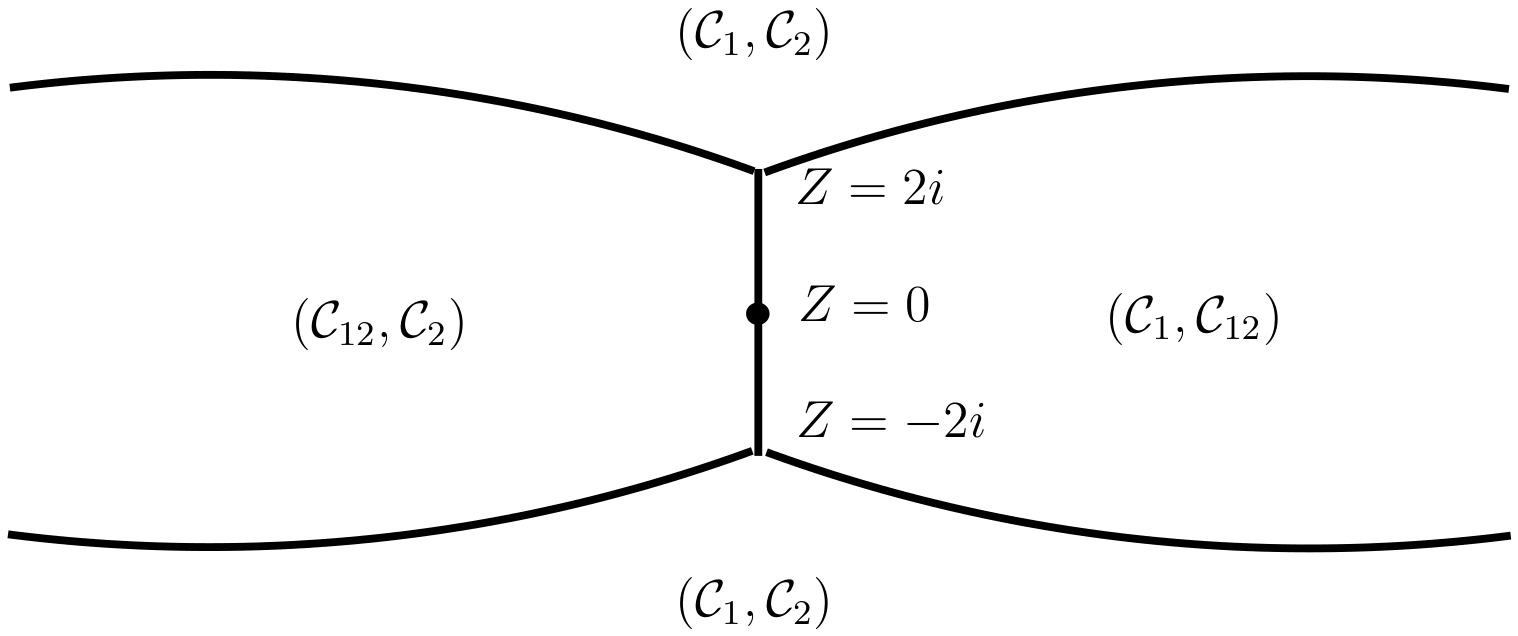
\includegraphics[width=4in]{figs/Fig13.png}
 \end{center}
\caption{\small $c(z_1 - z_2)$ 平面中 Stokes 墙的分布与针基。（原稿第 68 页）}
 \label{braidb}
\end{figure}

我们在图~\ref{braidb} 中画出针系的 Stokes 墙。参数空间中存在这样的区域：在其中针基由 $\CC_1$、$\CC_2$ 与 $\CC_{12}$ 中的任意两条构成（至多相差超势分支的选择）。区域两两沿 Stokes 墙相接，三个区域则在两个临界点重合的点 $Z=\pm 2i$ 处相遇。这是一般性特征；在这类一般问题中，总会存在复余维 $1$ 的轨迹，在其上两个临界点重合。在垂直于该轨迹的平面内，$\W$ 可以用单变量 $w$ 的简单三次函数 $\W = w^3 + \delta w$（带参数 $\delta$）来模拟；该函数有两个临界点，它们在 $\delta=0$ 时重合，此处三条 Stokes 墙相交。局部的 Stokes 行为是普适的；它对应于 Airy 函数的行为。

% [Tutor Note: 数学工具] $\W=w^3+\delta w$ 是两临界点碰撞的普适模型（余维 1 的 $A_2$ 型奇点）：$\delta=0$ 时三重临界点处有三条 Stokes 墙交汇，其局部构型由 $\W=w^3$ 的相位决定，相关 Stokes 乘子由 Airy 函数的渐近展开固定。记住这一点可省去逐题计算：任何"两临界点靠近"的局部问题，其编织矩阵的普适部分都是 Airy/Stokes 乘子，差别只在全局的 $q$ 幂次。

正如我们在第~\ref{fromth}~节的一般讨论中所解释的，$b\to 0$ 时积分的渐近行为在针基下最为清晰。就当前问题而言，图~\ref{braidb} 已经抓住了相关信息。图中共有四个区域：上下两个区域对应于我们在 $|Z|>>1$ 极限下看到的针系，中间两个区域对应于我们在 $|Z|<<1$ 极限下看到的针系。

\begin{figure}
 \begin{center}
     % >>> 原文图 14（原稿第 68 页）
  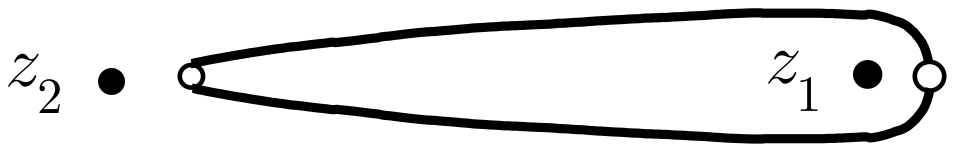
\includegraphics[width=2.5in]{figs/Fig14.png}
 \end{center}
\caption{\small 从 $z_2$ 附近的临界点（空心圆点）流向 $z_1$ 附近临界点（空心圆点）的两条 Morse 流。这两条流发生在略有不同的 ${\mathrm{Im}}\,Z$ 值处。（原稿第 68 页）}
 \label{braidc}
\end{figure}

公式 (\ref{furthox}) 或 (\ref{nurth}) 描述了编织矩阵 $B_{12}$，它把图~\ref{braidb} 顶部（此处的针是 $\CC_1$ 与 $\CC_2$）的区域与底部（此处的针同样是 $\CC_1$ 与 $\CC_2$）的区域联系起来。这个计算是我们凭观察作出的，而不是通过分析 Stokes 线得到的。在推导 (\ref{nurth}) 时，我们假定 $z_1$ 沿顺时针方向绕 $z_2$ 走了半圈；这相当于在图~\ref{braidb} 中取 $\mathrm{Re}\,Z>0$ 而从顶部移到底部。由图~\ref{braidb} 可见，在这一过程中我们会穿过两条 Stokes 线。这意味着，在针基下，编织矩阵 $B_{12}$ “分解”为两个基本操作的序列，每个基本操作与一条 Stokes 线相伴。每个基本操作都涉及一个梯度流：Bethe 根 $w$ 从 $z_2$ 右侧邻近的临界点流向 $z_1$ 右侧邻近的临界点。这样的流有两条，区别在于 $w$ 从 $z_1$ 上方还是下方经过。这两条流发生在略有不同的 $\mathrm{Im}\,Z$ 值处，如图~\ref{braidc} 所示。在式 (\ref{nurth}) 的公式 $B_{12}\tilde C_2=
(q^{-1/4}-q^{3/4})\tilde C_2+q^{1/4}\tilde C_1$ 中，右端的项 $q^{1/4}\tilde C_1$ 仅来自形式单值性，而另外两项则来自两个梯度流解的贡献。

% [Tutor Note: 易错点] “形式单值性”（formal monodromy）与梯度流贡献的分解是本题最易混淆处：$q^{1/4}\tilde C_1$ 项不来自任何实际流，算的是绕 $Z=0$ 一圈时对数分支的解析延拓；而 $(q^{-1/4}-q^{3/4})\tilde C_2$ 中的两项分别对应穿过两条 Stokes 线时的跳变。若把三项统统当作“流的贡献”，就会错误地预测应有三个临界点或三条流。核对时可用 $b\to0$ 的鞍点图像：只有真实临界点才给出指数小的贡献。

在小 $Z$ 区域，绕 $Z=0$ 的编织在针基下由三角矩阵表示：$\CC_{12}$ 是一个本征向量。这一事实有一般的理由：无论在 $Z \to 0$ 极限还是在 $b \to 0$ 极限下，沿 $\CC_{12}$ 的积分都小于沿任何其他链的积分。在任一极限下，沿 $\CC_{12}$ 的积分都由通常的鞍点近似控制，而与 $\CC_{12}$ 相伴的临界点正是 Morse 函数取最小值的那个临界点。因此 $\CC_{12}$ 必定是单值性的本征向量。对于任意数目的 $z$ 与 $w$，那些在某对非常接近的 $z_a$ 之间夹有一个 $w$ 的针集合，张成共形块的“小”本征空间，其中动量为 $- \frac{1}{2b}$ 的两个退化场融合为恒等场。

\subsubsection{第二个例子}\label{sec}

第二个有两个临界点的例子出现在有三个最小荷奇异磁单极子与一个 Bethe 根 $w$ 的情形。把奇异磁单极子置于 $z_1,z_2,z_3$，此时有三个显然可能的积分链：连接 $z_a$ 与 $z_b$ 的直线路径（对任意 $a,b$）。我们可以选取超势的分支，使得这三条链之和为零。

若这三点不共线，则上述定义是有意义的。此时 $z_a$ 的参数空间被分成两半：或者 $z_1$、$z_2$、$z_3$ 构成正向的三角形，或者构成负向的三角形。我们把两种情形下的三条自然链都记为 $\CC_{ab}^\pm$。于是
\begin{equation} \label{skeinc}
\CC^+_{12} + \CC^+_{23} + \CC^+_{31} = 0 \qquad \CC^-_{12} + \CC^-_{23} + \CC^-_{31} =0
\end{equation}
但这两组基在 $z_a$ 共线的轨迹两侧以有趣的方式相联系。

这样的轨迹有三条，每条对应三个 $z_a$ 中某一个从另外两个之间穿过。例如，若 $z_2$ 从 $z_1$ 与 $z_3$ 之间穿过，则 $\CC^+_{12}$ 与 $\CC^+_{23}$ 同 $\CC^-_{12}$ 与 $\CC^-_{23}$ 的关系仅仅是 $\W$ 的分支改变，而 $\CC^+_{13}$ 的变换则由 (\ref{skeinc}) 推出。

Bethe 方程
\begin{equation}\label{polz} \frac{1}{w-z_1}+\frac{1}{w-z_2}+\frac{1}{w-z_3} =0 \end{equation}
等价于关于 $w$ 的一个二次方程，因此它有两个解，对应于两个独立的针。这些针等价于连接某一对 $z$ 的路径中的两条，但具体出现哪两对取决于 $z$ 的选取。若各 $z$ 共线，则 Bethe 根位于相邻 $z$ 之间的线段上，而针与这些线段重合。例如，若 $z_2$ 位于 $z_1$ 与 $z_3$ 之间，则两个针是 $\CC^\pm_{12}$ 与 $\CC^\pm_{23}$（至多相差 $q$ 的幂次）。

与通常一样，连接 $z_a$ 与 $z_b$ 的针对应于相应的两个退化场融合为恒等场的共形块。关系式 (\ref{skeinc}) 对应于三个初级场中取两个融合为恒等场的三种不同方式之间的基本“拆接关系”（skein relation）。换言之，只要 $z_a$ 与 $z_b$ 靠得很近，就存在一条连接它们的针，它是 $z_a$ 与 $z_b$ 之编织的本征向量，而该编织矩阵是三角的。

\begin{figure}
 \begin{center}
     % >>> 原文图 15（原稿第 70 页）
  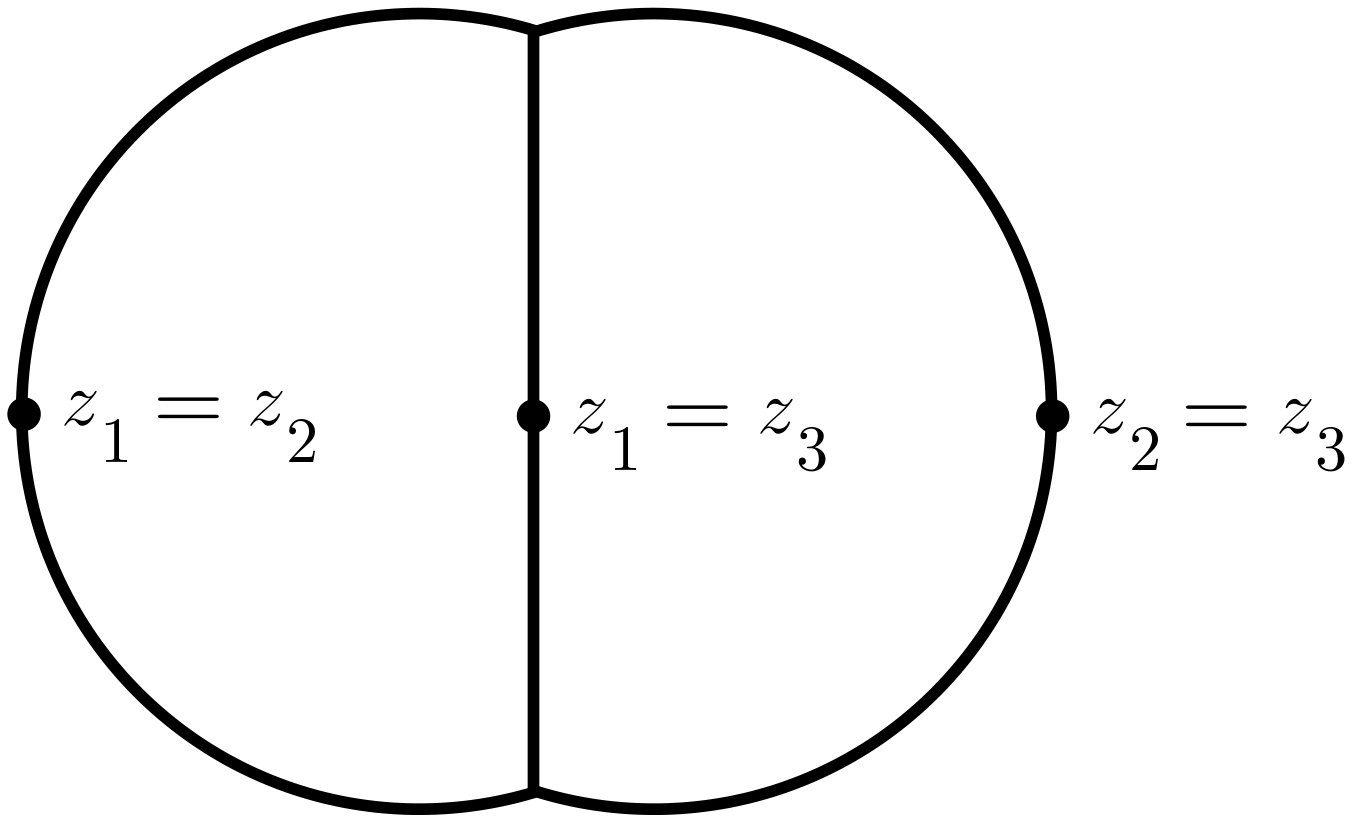
\includegraphics[width=3.5in]{figs/Fig15.png}
 \end{center}
\caption{\small 以 $z_1$、$z_2$、$z_3$ 为顶点的三角形形状空间中的 Stokes 墙分布。（原稿第 70 页）}
 \label{stok}
\end{figure}

我们在图~\ref{stok} 中画出这些 Stokes 墙。积分 $I_{ab}$ 可以容易地用超几何函数求出。

\subsection{最后一个例子}\label{fin}
还有一个例子既有启发性，又对理解一般图像很有用。这就是两个荷为 $1$ 的 $z_a$ 伴随着两个 $w_i$ 的情形。这只能在存在复对称性破缺时发生。容易看出，Bethe 方程 (\ref{normo}) 只有唯一的解。$Q$ 与 $K$ 的次数都是 $2$，因此 $P$ 的次数为 0，可以取为 1。由此得到一组线性方程，它们唯一地确定 $Q$ 中的系数。由于 Bethe 方程的解唯一，只有一个共形块，而编织 $z_a$ 时的单值性只能是乘以 $q$ 的某个函数。

% [Tutor Note: 易错点] 这里的 $P,Q,K$ 是 Bethe 拟设中用到的多项式（$Q=\prod(w-w_i)$ 等），“$\deg Q=\deg K=2$ 故 $\deg P=0$” 的计数依赖前文 (\ref{normo}) 的具体形式，不要把它当成一般结论。另外，“单值性只能是乘以 $q$ 的某个函数”之所以成立，是因为只有一个本征向量（一维表示）；若解不唯一，单值性就会是矩阵而非标量。

若 $z_1$ 与 $z_2$ 相距很远，即 $c(z_1 - z_2)$ 的绝对值很大，则 Bethe 方程的解容易描述：$w_1 \sim z_1 + 1/c$ 与 $w_2 \sim z_2 + 1/c$。存在一个显然的积分链：$w_1$ 与 $w_2$ 分别沿从 $z_1$ 与 $z_2$ 出发、朝 $c$ 方向伸向无穷的射线积分；这些射线在图~\ref{cyclesonetwo} 中被标为 $\CC_1$ 与 $\CC_2$。我们可以把这个链记为 $\CC = \CC_1 \times \CC_2$。

若 $Z = c(z_1 - z_2)$ 的虚部很大，则该问题的唯一针是 $\CC$ 的小形变。当我们形变 $Z$ 时，唯一的针会连续地形变。Morse 理论在这里相当有用：用手工验证 $\CC$ 在 $z_1$ 与 $z_2$ 编织之后回到自身是相当棘手的，因为这需要一次不能使 $\CC$ 保持简单乘积形式的围道形变；而针的演化恰好隐含地提供了这样的形变。同样，乍看之下远不明显的是，由 $w_1$ 与 $w_2$ 上的围道积分产生的共形块，会是 $Z$ 平面中具有阿贝尔单值性的简单函数。然而情形必定如此。

编织的效应在大 $c$ 下可以通过积分的鞍点估计容易地算出。在鞍点处，只要整个过程在大 $|Z|$ 下进行，$w_1 \sim z_1 + 1/c$ 与 $w_2 \sim z_2 + 1/c$ 就在整个编织过程中保持成立。$\W$ 的 Hessian 接近于单位矩阵的一个大的、与 $Z$ 无关的倍数（$\sim| c |^2$），因此大 $Z$ 下的编织相位由临界点处 $\exp(\W/b^2)$ 的取值控制。相关因子为
\begin{equation}
(z_1 - z_2)^{-b^{-2}/2} (w_1 - z_2)^{b^{-2}}(w_2 - z_1)^{b^{-2}}(w_1 - w_2)^{-2 b^{-2}} \sim (z_1 - z_2)^{-b^{-2}/2}.
\end{equation}
于是我们重新得到与两个 $z_a$ 荷为 $1$、不含 $w_i$ 的构型中相同的编织相位。

后一陈述将成为第~\ref{abdesc}~节构造有效阿贝尔描述的部分依据。在阿贝尔理论中，人们会预期两个对象的编织只依赖于它们荷的乘积。因此，两个荷均为 $-1$ 的对象（不带 $w$ 的 $z$）之间的编织，与两个荷均为 1 的对象（带 $w$ 的 $z$）之间的编织给出相同的结果。荷为 1 的对象与荷为 $-1$ 的对象之间的编织则不那么简单，因为正如我们在第~\ref{twop}~节所看到的，非平凡的梯度流会进入其中。

\subsection{存在对称性破缺的一般图像}\label{genpicture}
本节中，我们建立存在对称性破缺的一般图像。取对称性破缺参数 $c$ 为实的正数；考虑任意数目的奇异磁单极子，位于 $z_a$，$a=1,\dots,d$，以及任意数目的 Bethe 根 $w_i$，$i=1,\dots,q$。首先，我们把所有荷 $k_a$ 都取为 $1$。

我们可以手工构造一组积分链基。假定各 $z_a$ 的虚部互不相同，并按 $a'>a$ 时 $\mathrm{Im} (z_a- z_{a'}) >0$ 排序。我们定义从 $z_a$ 出发、平行于正实轴的射线 $\CC_a$。

我们的积分链将是乘积 $\CC_{a_1 a_2\cdots a_q} := 
\CC_{a_1} \times\CC_{a_2} \times \cdots \times \CC_{a_q}$，对应于 $q$ 个互不相同 $z$ 的每一个子集。这样得到 ${d \choose q}$ 条积分链，在大 $c$ 区域它们可以解释为针。确实，Bethe 方程
\begin{equation}
\sum_a \frac{1}{w_i - z_a} = c + \sum_{j \neq i} \frac{2}{w_i - w_j}
\end{equation}
在大 $c$ 时有近似解，其中每个 $w_i$ 近似等于 $z_{a_i}+1/c$，且当 $i\not=j$ 时 $a_i\not=a_j$。相应的针正是 $\CC_{a_1a_2\dots a_q}$。对所有 $q$ 求和，我们一共得到 $2^d$ 个临界点或共形块，正如所预期的那样。

在这组基下，辫群表示相当简单。我们让各 $z_a$ 在复平面中移动。Stokes 墙近似位于两个 $z_a$ 实部相等的轨迹处。当且仅当某个不带 $w_i$ 的 $z_a$ 从某个带 $w_i$ 的 $z_{a'}$ 右侧经过时，才会出现 Morse 流。由此产生的行为只涉及正在交叉的那两个 $z$，并且正是我们在第~\ref{twop}~节详细分析过的内容。当 $z_a$ 穿过 $z_{a'}$ 时，编织矩阵只非平凡地作用于 $\CC_a$ 与 $\CC_{a'}$（以及任何包含其中之一或两者的链 $\CC_{a_1a_2\dots a_q}$），并取与 (\ref{nurth}) 相同的形式。如图~\ref{braidc} 所示，这一过程的编织矩阵可以解释为源于一对 Morse 理论流。验证辫群关系成立是繁琐的，但却是初等的；它们理应成立。
